\heada{MESH}{BLOCk}
\hspace{1.0cm}{{ bloc (Line in 1,2,or3-D) \hfill}} \\{\smallskip}
\hspace{1.4cm}{{ type,r-inc,,node1,[elmt1,mat,r-skip],b-type \hfill}}
\\{\smallskip}
\hspace{1.8cm}{{ 1,x1,y1,z1 (only ndm coordinates required) \hfill}}
\\{\smallskip}
\hspace{1.8cm}{{ 2,x2,y2,z2 \hfill}} \\{\smallskip}
\hspace{1.4cm}{{ etc.,blank record after all nodes are input \hfill}}
\\{\smallskip}
\hspace{1.4cm}{{ bloc (Surface in 2 or 3-D) \hfill}} \\{\smallskip}
\hspace{1.4cm}{{ type,r-inc,s-inc,node1,[elmt1,mat,r-skip],b-type \hfill}}
\\{\smallskip}
\hspace{1.8cm}{{ 1,x1,y1,z1 (only ndm coordinates required) \hfill}}
\\{\smallskip}
\hspace{1.8cm}{{ 2,x2,y2,z2 \hfill}} \\{\smallskip}
\hspace{1.4cm}{{ etc.,blank record after all nodes are input \hfill}}
\\{\smallskip}
\hspace{1.4cm}{{ bloc (3-D Solid) \hfill}} \\{\smallskip}
\hspace{1.4cm}{{ type,r-inc,s-inc,t-inc,node1,[elmt1,mat],b-type \hfill}}
\\{\smallskip}
\hspace{1.8cm}{{ 1,x1,y1,z1 \hfill}} \\{\smallskip}
\hspace{1.8cm}{{ 2,x2,y2,z2 \hfill}} \\{\smallskip}
\hspace{1.4cm}{{ etc.,blank record after all nodes are input \hfill}}
\headb

The {\tt BLOC}k data input segment is used to generate:
\begin{enumerate}
\item 2-node line elements in 1, 2, or 3-D.
\item 4 to 9-node quadrilateral elements in 2 or 3-D.
\item 3 or 6-node triangles in 2 or 3-D.  For the 3-node
elements alternative diagonal directions may be specified as indicated below.
\item 8-node hexahedra (bricks) in 3-D.
\item 4-node tetrahedra in 3-D.
\item Nodes only in 1, 2 or 3-D patches.
\end{enumerate}

The patch of nodes and triangular or quadrilateral elements
defined by {\tt BLOC}k is developed from a master
element which is defined by an isoparametric 4 to 9
node mapping function in terms of the two natural coordinates,
r (or $\xi_1$) and s (or $\xi_2$), respectively.
The node numbers on the master element of each
patch defined by {\tt BLOC}k are specified according to Figure \ref{blk2d}.
The four corner nodes of the master element must be
specified, the mid-point and central nodes are optional.
The spacing between the r-increments and s-increments
may be varied by an off-center placement of mid-side and
central nodes.  Thus, it is possible to concentrate
nodes and elements into one corner of the patch generated by
{\tt BLOC}k.  The mid-nodes must lie within the central-half of
the r-direction and the s-direction to keep the isoparametric mapping
single valued for all (r,s) points.
For a line patch, the nodes and 2 node elements are
defined from a 1-2 master linear line patch or a 1-3-2 master
quadratic line patch.  The {\it s-inc} parameter must be 0 for this option.
For a 3-D solid the patch is described by an 8 to 27-node
master solid element where the corner nodes are
required and mid-edge/side nodes are optional, as is the
center node (numbering for nodes is shown in Figures \ref{blk3da}, \ref{blk3db}
and \ref{blk3dc}).

The location of nodes on boundaries of adjacent patches should match
unless a contact problem is used to determine interactions between
bodies.
The {\tt TIE} command is used to merge adjacent patches.

\begin{figure}[ht!]
\begin{center}
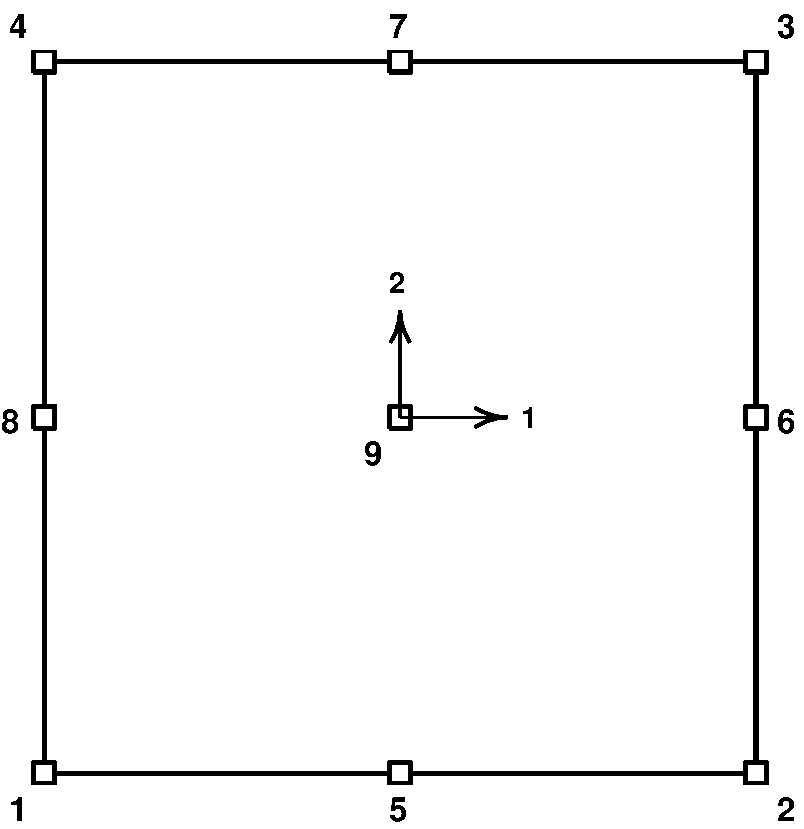
\includegraphics[width=3.1in]{../lmesh/block}
\caption{Node Specification on 2D Master Block.  \label{blk2d} }
\end{center}
\end{figure}

The data parameters are defined in Tables \ref{tblkn} and \ref{tblkt}.

\begin{table}
\begin{center}
\begin{tabular}{r l}
\it type   &-- Master node coordinate type ({\it cart, pola,} or {\it sphe}). \\
\it r-inc  &-- Number of nodal increments to be generated along \\
           &\quad r-direction of the patch. \\
\it s-inc  &-- Number of nodal increments to be generated along \\
           &\quad s-direction of the patch. \\
\it t-inc  &-- Number of nodal increments to be generated along \\
           &\quad t-direction of the patch (N.B. Input for 3-d blocks only). \\
\it node1  &-- Number to be assigned to first generated node in \\
           &\quad patch.  First node is located at same location \\
           &\quad as master node 1. \\
\it elmt1  &-- Number to be assigned to first element generated in \\
           &\quad patch. \\
\it matl   &-- Material identifier to be assigned to all generated elements \\
           &\quad elements in patch. \\
\it r-skip &-- For surfaces, number of nodes to skip between end of \\
           &\quad an r-line and start of next r-line (default = 1) \\
           &\quad (N.B. Not input for 3-d block). \\
\end{tabular}
\end{center}
\caption{Block Numbering Data}
\label{tblkn}
\end{table}
\begin{table}
\begin{center}
\begin{tabular}{r l}
\it b-type &=0: 4-node elements on surface patch; \\
           &\qquad 2-node elements on a line; \\
           &=1: 3-node triangles (diagonals in 1-3 direction of block); \\
           &=2: 3-node triangles (diagonals in 2-4 direction of block); \\
           &=3: 3-node triangles (diagonals alternate 1-3 then 2-4); \\
           &=4: 3-node triangles (diagonals alternate 2-4 then 1-3); \\
           &=5: 3-node triangles (diagonals in union-jack pattern); \\
           &=6: 3-node triangles (diagonals in inverse union-jack pattern); \\
           &=7: 6-node triangles (similar to =1 orientation); \\
           &=8: 8-node quadrilaterals ({\it r-inc} and {\it s-inc} must be even \\
		   &\qquad numbers);  N.B. Interior node generated but not used; \\
           &=9: 9-node quadrilaterals ({\it r-inc} and {\it s-inc} must be even \\
           &\qquad numbers); \\
           &=10: 8-node hexahedra (bricks). \\
           &=11: 4-node tetrahedra.
\end{tabular}
\end{center}
\caption{Block Type Data}
\label{tblkt}
\end{table}

When using the {\tt BLOC}k command one may enter zero for the
total number of nodes and elements on the {\tt FEAPpv} control
record.  {\tt BLOC}k will automatically generate the correct
number of nodes and elements.
If it is desired to use block to generate nodal coordinates only, the
value of {\it elmt1} should be entered as a negative number.

\begin{figure}[ht!]
\center {\hfil 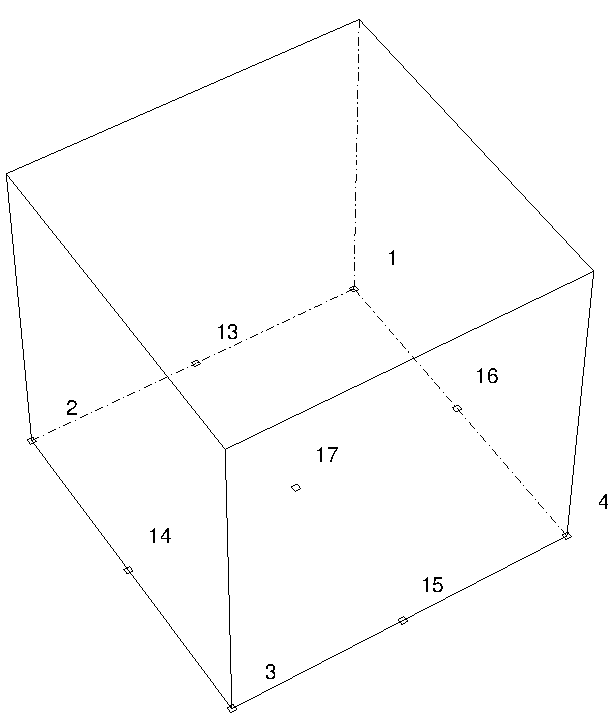
\includegraphics[width=3.1in]{figs/blk3a} \hfil}
\caption{Node Specification on 3D Master Block.}
\label{blk3da}
\end{figure}

\begin{figure}[ht!]
\center {\hfil 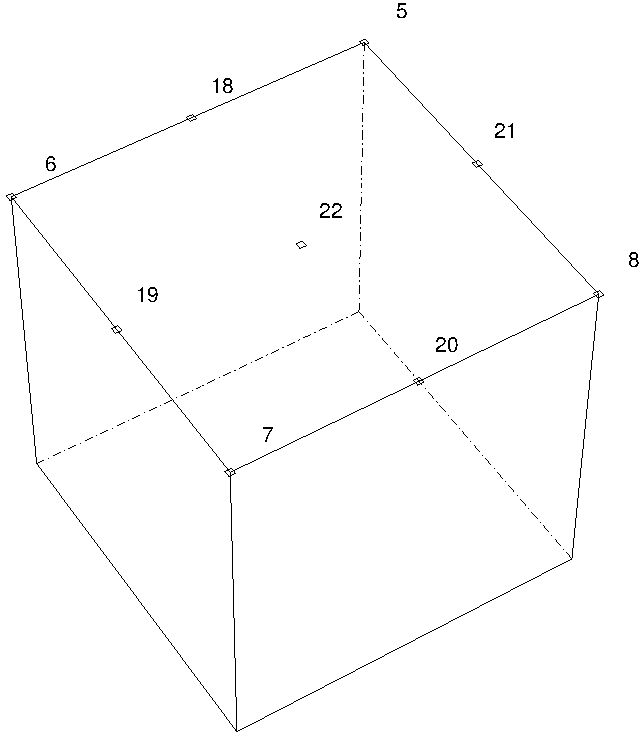
\includegraphics[width=3.1in]{figs/blk3b} \hfil}
\caption{Node Specification on 3D Master Block.}
\label{blk3db}
\end{figure}

\begin{figure}[ht!]
\center {\hfil 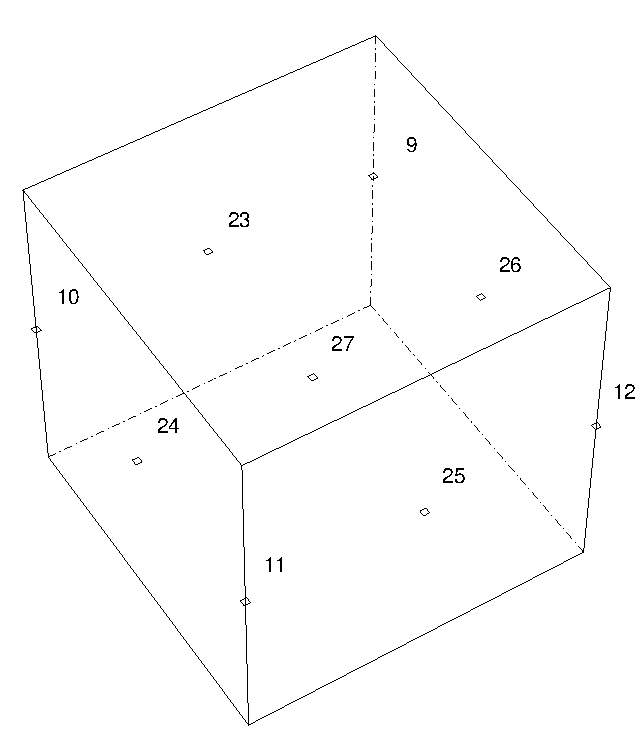
\includegraphics[width=3.1in]{figs/blk3c} \hfil}
\caption{Node Specification on 3D Master Block.}
\label{blk3dc}
\end{figure}


\vspace*{3.1in}

\pagebreak
